% Options for packages loaded elsewhere
\PassOptionsToPackage{unicode,linktoc=all}{hyperref}
\PassOptionsToPackage{hyphens}{url}
\PassOptionsToPackage{dvipsnames,svgnames,x11names}{xcolor}
%
\documentclass[
  letterpaper,
]{book}

\usepackage{amsmath,amssymb}
\usepackage{lmodern}
\usepackage{iftex}
\ifPDFTeX
  \usepackage[T1]{fontenc}
  \usepackage[utf8]{inputenc}
  \usepackage{textcomp} % provide euro and other symbols
\else % if luatex or xetex
  \usepackage{unicode-math}
  \defaultfontfeatures{Scale=MatchLowercase}
  \defaultfontfeatures[\rmfamily]{Ligatures=TeX,Scale=1}
\fi
% Use upquote if available, for straight quotes in verbatim environments
\IfFileExists{upquote.sty}{\usepackage{upquote}}{}
\IfFileExists{microtype.sty}{% use microtype if available
  \usepackage[]{microtype}
  \UseMicrotypeSet[protrusion]{basicmath} % disable protrusion for tt fonts
}{}
\makeatletter
\@ifundefined{KOMAClassName}{% if non-KOMA class
  \IfFileExists{parskip.sty}{%
    \usepackage{parskip}
  }{% else
    \setlength{\parindent}{0pt}
    \setlength{\parskip}{6pt plus 2pt minus 1pt}}
}{% if KOMA class
  \KOMAoptions{parskip=half}}
\makeatother
\usepackage{xcolor}
\usepackage[top=30mm,left=20mm,heightrounded]{geometry}
\usepackage[normalem]{ulem}
\setlength{\emergencystretch}{3em} % prevent overfull lines
\setcounter{secnumdepth}{5}
% Make \paragraph and \subparagraph free-standing
\ifx\paragraph\undefined\else
  \let\oldparagraph\paragraph
  \renewcommand{\paragraph}[1]{\oldparagraph{#1}\mbox{}}
\fi
\ifx\subparagraph\undefined\else
  \let\oldsubparagraph\subparagraph
  \renewcommand{\subparagraph}[1]{\oldsubparagraph{#1}\mbox{}}
\fi


\providecommand{\tightlist}{%
  \setlength{\itemsep}{0pt}\setlength{\parskip}{0pt}}\usepackage{longtable,booktabs,array}
\usepackage{calc} % for calculating minipage widths
% Correct order of tables after \paragraph or \subparagraph
\usepackage{etoolbox}
\makeatletter
\patchcmd\longtable{\par}{\if@noskipsec\mbox{}\fi\par}{}{}
\makeatother
% Allow footnotes in longtable head/foot
\IfFileExists{footnotehyper.sty}{\usepackage{footnotehyper}}{\usepackage{footnote}}
\makesavenoteenv{longtable}
\usepackage{graphicx}
\makeatletter
\def\maxwidth{\ifdim\Gin@nat@width>\linewidth\linewidth\else\Gin@nat@width\fi}
\def\maxheight{\ifdim\Gin@nat@height>\textheight\textheight\else\Gin@nat@height\fi}
\makeatother
% Scale images if necessary, so that they will not overflow the page
% margins by default, and it is still possible to overwrite the defaults
% using explicit options in \includegraphics[width, height, ...]{}
\setkeys{Gin}{width=\maxwidth,height=\maxheight,keepaspectratio}
% Set default figure placement to htbp
\makeatletter
\def\fps@figure{htbp}
\makeatother

\makeatletter
\makeatother
\makeatletter
\@ifpackageloaded{bookmark}{}{\usepackage{bookmark}}
\makeatother
\makeatletter
\@ifpackageloaded{caption}{}{\usepackage{caption}}
\AtBeginDocument{%
\ifdefined\contentsname
  \renewcommand*\contentsname{Table of contents}
\else
  \newcommand\contentsname{Table of contents}
\fi
\ifdefined\listfigurename
  \renewcommand*\listfigurename{List of Figures}
\else
  \newcommand\listfigurename{List of Figures}
\fi
\ifdefined\listtablename
  \renewcommand*\listtablename{List of Tables}
\else
  \newcommand\listtablename{List of Tables}
\fi
\ifdefined\figurename
  \renewcommand*\figurename{Figure}
\else
  \newcommand\figurename{Figure}
\fi
\ifdefined\tablename
  \renewcommand*\tablename{Table}
\else
  \newcommand\tablename{Table}
\fi
}
\@ifpackageloaded{float}{}{\usepackage{float}}
\floatstyle{ruled}
\@ifundefined{c@chapter}{\newfloat{codelisting}{h}{lop}}{\newfloat{codelisting}{h}{lop}[chapter]}
\floatname{codelisting}{Listing}
\newcommand*\listoflistings{\listof{codelisting}{List of Listings}}
\makeatother
\makeatletter
\@ifpackageloaded{caption}{}{\usepackage{caption}}
\@ifpackageloaded{subcaption}{}{\usepackage{subcaption}}
\makeatother
\makeatletter
\@ifpackageloaded{tcolorbox}{}{\usepackage[many]{tcolorbox}}
\makeatother
\makeatletter
\@ifundefined{shadecolor}{\definecolor{shadecolor}{rgb}{.97, .97, .97}}
\makeatother
\makeatletter
\makeatother
\ifLuaTeX
  \usepackage{selnolig}  % disable illegal ligatures
\fi
\IfFileExists{bookmark.sty}{\usepackage{bookmark}}{\usepackage{hyperref}}
\IfFileExists{xurl.sty}{\usepackage{xurl}}{} % add URL line breaks if available
\urlstyle{same} % disable monospaced font for URLs
\hypersetup{
  pdftitle={Confounders},
  pdfauthor={Joaquin Saposnik},
  colorlinks=true,
  linkcolor={blue},
  filecolor={Maroon},
  citecolor={Blue},
  urlcolor={Blue},
  pdfcreator={LaTeX via pandoc}}

\title{Confounders}
\author{Joaquin Saposnik}
\date{5/10/2022}

\begin{document}
\frontmatter
\maketitle
\ifdefined\Shaded\renewenvironment{Shaded}{\begin{tcolorbox}[interior hidden, breakable, enhanced, frame hidden, borderline west={3pt}{0pt}{shadecolor}, sharp corners, boxrule=0pt]}{\end{tcolorbox}}\fi

\renewcommand*\contentsname{Table of contents}
{
\hypersetup{linkcolor=}
\setcounter{tocdepth}{5}
\tableofcontents
}
\mainmatter
\bookmarksetup{startatroot}

\hypertarget{introducciuxf3n}{%
\chapter*{Introducción}\label{introducciuxf3n}}
\addcontentsline{toc}{chapter}{Introducción}

Se desea hacer un modelo lineal simple entre las variables del dataset
de seguros registrando la amplitud del efecto en la forma de los
coeficientes que acompañana a la o las variables independientes. Para
eso se probarán y compararán distintos modelos identificando el mejor de
ellos.

\hypertarget{limpieza-y-adecuaciuxf3n-de-los-datos}{%
\section*{Limpieza y adecuación de los
datos}\label{limpieza-y-adecuaciuxf3n-de-los-datos}}
\addcontentsline{toc}{section}{Limpieza y adecuación de los datos}

El dataset provisto posee 7 columnas, con variables categóricas (sexo,
fumador, región) y numéricas (edad, índice de masa corporal, hijes,
gastos de seguro médico). Se verificó que la importación de los datos
sea correcta y se eliminaron filas repetidas. Se agregó 1 nueva columna
llamada ``salud'':

\begin{itemize}
\tightlist
\item
  \uline{\textbf{Salud:}} considerando la obesidad de una persona como
  el BMI mayor o igual a 30 y si esta persona es fumadora, separa entre
  personas Obesas Fumadoras (OF), Obesas No Fumadoras (ONF), No Obesas
  Fumadoras (NOF) y No Obesas No Fumadoras (NONF).
\end{itemize}

\hypertarget{modelo-lineal-simple-n-1}{%
\section*{Modelo lineal simple N° 1}\label{modelo-lineal-simple-n-1}}
\addcontentsline{toc}{section}{Modelo lineal simple N° 1}

Se realizaron dos variaciones de un modelo lineal simple (ver
Figure~\ref{fig-modelo1_simple}) teniendo en cuenta los gastos de una
persona en función de su edad. Se utilizaron las fórmulas:

\begin{itemize}
\item
  \uline{\textbf{Modelo 1.1:}} \(y\) \textasciitilde{} \(x_1\)
\item
  \uline{\textbf{Modelo 1.2:}} \(y\) \textasciitilde{} \(x_1 - 1\)
\end{itemize}

Reemplazando: \(y = charges,\) \(x_1 = age\).

\begin{figure}

{\centering 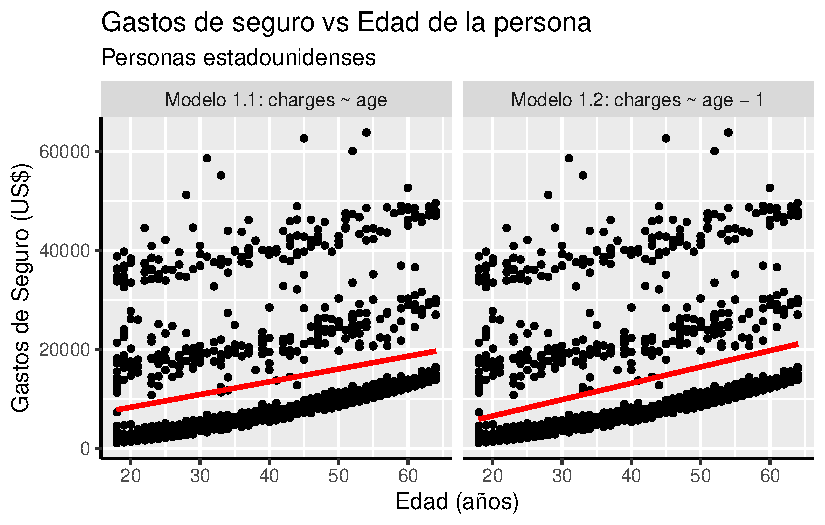
\includegraphics{./index_files/figure-pdf/fig-modelo1_simple-1.pdf}

}

\caption{\label{fig-modelo1_simple}Modelo lineal simple N° 1 - Gastos vs
Edad.}

\end{figure}

Se observó que el Modelo 1.2 tiene mejor estimación que el Modelo 1.1 ya
que las edades no comienzan en 0; y al suprimir la ordenada al origen
del modelo, se obtiene una mejor tendencia. Sin embargo, ninguno de
ambos modelos se ajusta debidamente a los datos ya que hay otros
factores que influyen en los gastos de una persona como su estado de
salud. Las estadísticas de los Modelos 1.1 (ver
Table~\ref{tbl-stats_modelo1.1_simple}) y 1.2 (ver
Table~\ref{tbl-stats_modelo1.2_simple}) demuestran que efectivamente no
son ideales.

\hypertarget{tbl-stats_modelo1.1_simple}{}
\begin{longtable}[]{@{}ccccccl@{}}
\caption{\label{tbl-stats_modelo1.1_simple}Estadísticas del modelo
lineal simple N° 1.1.}\tabularnewline
\toprule()
~ & charges & & & & & \\
\midrule()
\endfirsthead
\toprule()
~ & charges & & & & & \\
\midrule()
\endhead
Predictors & p & Statistic & Estimates & standardized std. Error & std.
Error & std. Beta \\
(Intercept) & \textbf{6.95e-04} & 3.40 & 3190.02 & 0.03 & 938.40 &
0.00 \\
age & \textbf{6.98e-29} & 11.42 & 257.23 & 0.03 & 22.53 & 0.30 \\
Observations & 1337 & & & & & \\
R\textsuperscript{2} / R\textsuperscript{2} adjusted & 0.089 / 0.088 & &
& & & \\
\bottomrule()
\end{longtable}

\hypertarget{tbl-stats_modelo1.2_simple}{}
\begin{longtable}[]{@{}ccccccl@{}}
\caption{\label{tbl-stats_modelo1.2_simple}Estadísticas del modelo
lineal simple N° 1.2.}\tabularnewline
\toprule()
~ & charges & & & & & \\
\midrule()
\endfirsthead
\toprule()
~ & charges & & & & & \\
\midrule()
\endhead
Predictors & p & Statistic & Estimates & standardized std. Error & std.
Error & std. Beta \\
age & \textbf{5.68e-256} & 43.21 & 329.33 & 0.03 & 7.62 & 0.30 \\
Observations & 1337 & & & & & \\
R\textsuperscript{2} / R\textsuperscript{2} adjusted & 0.583 / 0.583 & &
& & & \\
\bottomrule()
\end{longtable}

\hypertarget{modelo-lineal-simple-n-2}{%
\section*{Modelo lineal simple N° 2}\label{modelo-lineal-simple-n-2}}
\addcontentsline{toc}{section}{Modelo lineal simple N° 2}

Para mejorar la estimación de los gastos, se procede a cambiar el
modeloagregando la variable ``salud'' que posee 4 posibles estados de
salud (ver Figure~\ref{fig-modelo2_simple}). Se utilizan los modelos:

\begin{itemize}
\item
  \uline{\textbf{Modelos 2.1:}} \(y\) \textasciitilde{} \(x_1 + x_2\)
\item
  \uline{\textbf{Modelos 2.2:}} \(y\) \textasciitilde{}
  \(x_1 + x_2 - 1\)
\end{itemize}

Reemplazando: \(y = charges,\) \(x_1 = age,\) \(x_2 = salud\).

\begin{figure}

{\centering 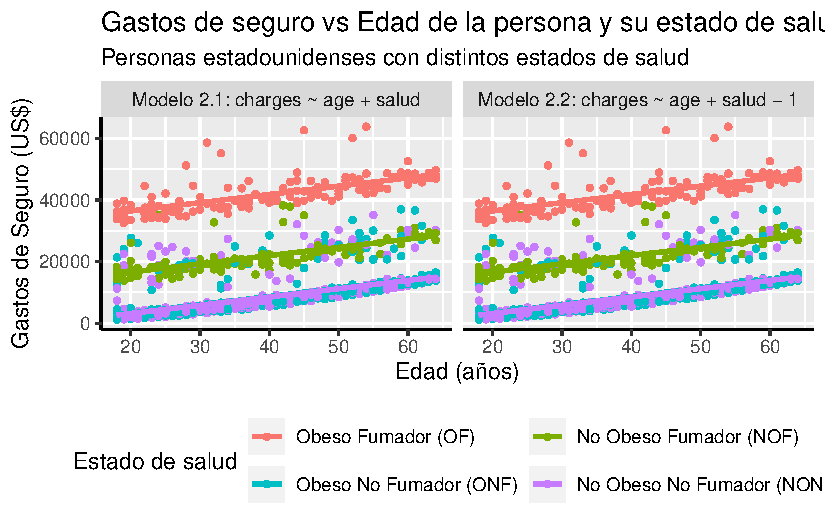
\includegraphics{./index_files/figure-pdf/fig-modelo2_simple-1.pdf}

}

\caption{\label{fig-modelo2_simple}Modelo lineal simple N° 2 - Gastos vs
Edad y Salud.}

\end{figure}

Se observa que los nuevos modelos tienen mejores estimaciones para los
distintos grupos de personas según su estado de salud, siendo mucho
mejor el Modelo 2.2 según la comparación de las estadísticas de los
modelos (Modelo 2.1, ver Table~\ref{tbl-stats_modelo2_simple} y Modelo
2.2, ver Table~\ref{tbl-stats_modelo2_2_simple}).

\hypertarget{tbl-stats_modelo2_simple}{}
\begin{longtable}[]{@{}ccccccl@{}}
\caption{\label{tbl-stats_modelo2_simple}Estadísticas del modelo lineal
simple N° 2.1.}\tabularnewline
\toprule()
~ & charges & & & & & \\
\midrule()
\endfirsthead
\toprule()
~ & charges & & & & & \\
\midrule()
\endhead
Predictors & p & Statistic & Estimates & standardized std. Error & std.
Error & std. Beta \\
(Intercept) & \textbf{9.73e-114} & 25.04 & 9523.57 & 0.01 & 380.29 &
0.56 \\
age & \textbf{2.19e-151} & 29.99 & 267.72 & 0.01 & 8.93 & 0.31 \\
salud {[}linear{]} & \textbf{0.00e+00} & -82.82 & -25286.22 & 0.03 &
305.33 & -2.09 \\
salud {[}quadratic{]} & \textbf{1.34e-165} & 31.80 & 9851.18 & 0.03 &
309.77 & 0.81 \\
salud {[}cubic{]} & \textbf{3.48e-06} & 4.66 & 1466.13 & 0.03 & 314.62 &
0.12 \\
Observations & 1337 & & & & & \\
R\textsuperscript{2} / R\textsuperscript{2} adjusted & 0.858 / 0.858 & &
& & & \\
\bottomrule()
\end{longtable}

\hypertarget{tbl-stats_modelo2_2_simple}{}
\begin{longtable}[]{@{}ccccccl@{}}
\caption{\label{tbl-stats_modelo2_2_simple}Estadísticas del modelo
lineal simple N° 2.2.}\tabularnewline
\toprule()
~ & charges & & & & & \\
\midrule()
\endfirsthead
\toprule()
~ & charges & & & & & \\
\midrule()
\endhead
Predictors & p & Statistic & Estimates & standardized std. Error & std.
Error & std. Beta \\
age & \textbf{2.19e-151} & 29.99 & 267.72 & 0.01 & 8.93 & 0.31 \\
saludOF & \textbf{0.00e+00} & 60.31 & 31083.83 & 0.03 & 515.40 & 2.34 \\
saludNOF & \textbf{1.32e-87} & 21.41 & 11235.67 & 0.03 & 524.89 &
0.70 \\
saludONF & \textbf{7.98e-07} & -4.96 & -2039.70 & 0.02 & 411.27 &
-0.40 \\
saludNONF & \textbf{3.91e-08} & -5.53 & -2185.51 & 0.02 & 395.41 &
-0.41 \\
Observations & 1337 & & & & & \\
R\textsuperscript{2} / R\textsuperscript{2} adjusted & 0.936 / 0.936 & &
& & & \\
\bottomrule()
\end{longtable}

\hypertarget{modelo-lineal-simple-n-3}{%
\section*{Modelo lineal simple N° 3}\label{modelo-lineal-simple-n-3}}
\addcontentsline{toc}{section}{Modelo lineal simple N° 3}

Se analizó una última serie de modelos (ver
Figure~\ref{fig-modelo3_simple}) para comprobar si pueden mejorar la
estimación del Modelo 2.2 (ver Table~\ref{tbl-stats_modelo2_2_simple}).
Se utilizaron las siguientes fórmulas:

\begin{itemize}
\item
  \uline{\textbf{Modelos 3.1:}} \(y\) \textasciitilde{} \(x_1 * x_2\)
\item
  \uline{\textbf{Modelos 3.2:}} \(y\) \textasciitilde{}
  \(x_1 * x_2 - 1\)
\end{itemize}

Reemplazando: \(y = charges,\) \(x_1 = age,\) \(x_2 = salud\).

\begin{figure}

{\centering 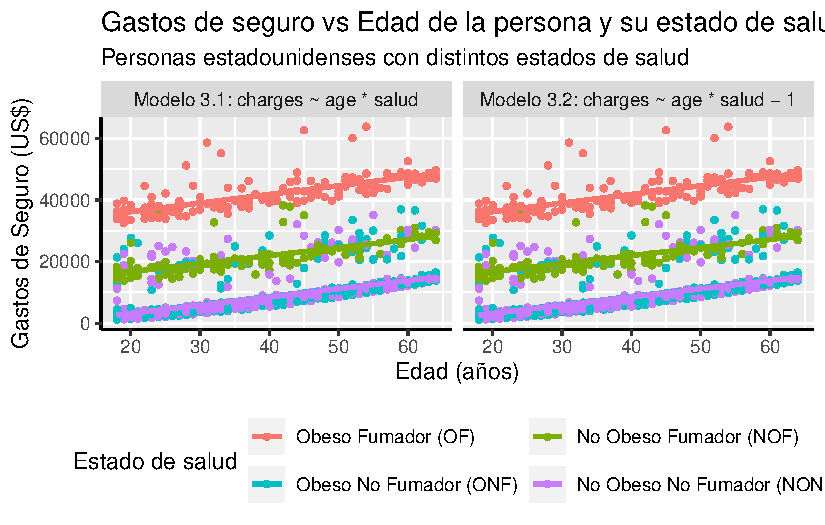
\includegraphics{./index_files/figure-pdf/fig-modelo3_simple-1.pdf}

}

\caption{\label{fig-modelo3_simple}Modelo lineal simple N° 3 - Gastos vs
Edad y Salud.}

\end{figure}

Al no poder visualizar un cambio significativo con respecto al gráfico
del Modelo 2.2 (ver Figure~\ref{fig-modelo2_simple}), se procede a
observar las estadísticas (Modelo 3.1 ver
Table~\ref{tbl-stats_modelo3_simple}, y Modelo 3.2 ver
Table~\ref{tbl-stats_modelo3_2_simple}.

\hypertarget{tbl-stats_modelo3_simple}{}
\begin{longtable}[]{@{}ccccccl@{}}
\caption{\label{tbl-stats_modelo3_simple}Estadísticas del modelo lineal
simple N° 3.1.}\tabularnewline
\toprule()
~ & charges & & & & & \\
\midrule()
\endfirsthead
\toprule()
~ & charges & & & & & \\
\midrule()
\endhead
Predictors & p & Statistic & Estimates & standardized std. Error & std.
Error & std. Beta \\
(Intercept) & \textbf{2.00e-82} & 20.66 & 9481.83 & 0.01 & 459.05 &
0.56 \\
age & \textbf{6.34e-106} & 23.98 & 268.72 & 0.01 & 11.20 & 0.31 \\
salud {[}linear{]} & \textbf{2.59e-134} & -27.78 & -24943.04 & 0.03 &
897.83 & -2.09 \\
salud {[}quadratic{]} & \textbf{4.45e-24} & 10.32 & 9476.10 & 0.03 &
918.11 & 0.81 \\
salud {[}cubic{]} & 6.05e-02 & 1.88 & 1762.24 & 0.03 & 937.94 & 0.12 \\
age * salud {[}linear{]} & 6.88e-01 & -0.40 & -8.75 & 0.03 & 21.77 &
-0.01 \\
age * salud {[}quadratic{]} & 6.66e-01 & 0.43 & 9.67 & 0.03 & 22.41 &
0.01 \\
age * salud {[}cubic{]} & 7.36e-01 & -0.34 & -7.75 & 0.03 & 23.03 &
-0.01 \\
Observations & 1337 & & & & & \\
R\textsuperscript{2} / R\textsuperscript{2} adjusted & 0.858 / 0.858 & &
& & & \\
\bottomrule()
\end{longtable}

\hypertarget{tbl-stats_modelo3_2_simple}{}
\begin{longtable}[]{@{}ccccccl@{}}
\caption{\label{tbl-stats_modelo3_2_simple}Estadísticas del modelo
lineal simple N° 3.2.}\tabularnewline
\toprule()
~ & charges & & & & & \\
\midrule()
\endfirsthead
\toprule()
~ & charges & & & & & \\
\midrule()
\endhead
Predictors & p & Statistic & Estimates & standardized std. Error & std.
Error & std. Beta \\
age & \textbf{6.34e-106} & 23.98 & 268.72 & 0.01 & 11.20 & 0.31 \\
saludOF & \textbf{7.27e-133} & 27.59 & 30558.13 & 0.03 & 1107.51 &
2.34 \\
saludNOF & \textbf{4.73e-21} & 9.58 & 11503.36 & 0.03 & 1201.26 &
0.70 \\
saludONF & \textbf{5.11e-04} & -3.48 & -2015.80 & 0.02 & 578.67 &
-0.40 \\
saludNONF & \textbf{4.88e-04} & -3.50 & -2118.37 & 0.02 & 605.99 &
-0.41 \\
age * salud L & 6.88e-01 & -0.40 & -8.75 & 0.03 & 21.77 & -0.01 \\
age * salud Q & 6.66e-01 & 0.43 & 9.67 & 0.03 & 22.41 & 0.01 \\
age * salud C & 7.36e-01 & -0.34 & -7.75 & 0.03 & 23.03 & -0.01 \\
Observations & 1337 & & & & & \\
R\textsuperscript{2} / R\textsuperscript{2} adjusted & 0.936 / 0.935 & &
& & & \\
\bottomrule()
\end{longtable}

Puede verse que el Modelo 3.2 (ver
Table~\ref{tbl-stats_modelo3_2_simple}) tiene muy buenas estimaciones
con respecto al Modelo 3.1 (ver Table~\ref{tbl-stats_modelo3_simple}). A
su vez, si comparamos los Modelos 2.2 (ver
Table~\ref{tbl-stats_modelo2_2_simple}) y 3.2, se observa que son
prácticamente idénticos siendo ligeramente mejor el Modelo 2.2.

\hypertarget{conclusiones}{%
\section*{Conclusiones}\label{conclusiones}}
\addcontentsline{toc}{section}{Conclusiones}

Se decide optar por usar el Modelo 2.2 (ver
Figure~\ref{fig-modelo2_simple} y
Table~\ref{tbl-stats_modelo2_2_simple}) ya que tiene una mejor
estimación para los gastos de las personas según su edad y estado de
salud.


\backmatter

\end{document}
